\documentclass[acmtog]{acmart}

% remove the stuff template info we don't want
\settopmatter{printacmref=false}
\renewcommand\footnotetextcopyrightpermission[1]{}
\pagestyle{plain}

\makeatletter
\renewcommand\@formatdoi[1]{\ignorespaces}
\makeatother

\authorsaddresses{}
\acmDOI{}

\fancyfoot{}
%

\usepackage{booktabs} % For formal tables
\usepackage{graphicx}
\usepackage[export]{adjustbox}
\usepackage{float}
\usepackage{natbib}

% TOG prefers author-name bib system with square brackets
\citestyle{acmauthoryear}
\setcitestyle{numbers}

\usepackage[ruled]{algorithm2e} % For algorithms
\renewcommand{\algorithmcfname}{ALGORITHM}

\SetAlFnt{\small}
\SetAlCapFnt{\small}
\SetAlCapNameFnt{\small}
\SetAlCapHSkip{0pt}
\IncMargin{-\parindent}

\begin{document}

\title{Automated Playlist Generation}

\author{Kade Keith}
\affiliation{ \institution{Stanford University} }
\email{kade@stanford.edu}
\author{Demetrios Fassois}
\affiliation{ \institution{Stanford University} }
\email{dimifass@stanford.edu}

\begin{abstract}
Our project explores generating music playlists based on a song or set of seed songs using diverse features ranging from lyrical sentiment to song popularity. We approach the problem as both a graph problem and as a classification problem, and evaluate our results based on real human-curated playlists. We find that our feature set and models perform the task well and that lyrical content in particular is a good indicator for playlist generation.
\end{abstract}

\maketitle
\thispagestyle{empty}

\section{Introduction}

With the growth of music streaming services, there are now more songs than ever at music listeners fingertips. Because of this growth, the art of constructing playlists has become increasingly challenging, and discovering new music the in the expanse of choices is a daunting task. For this reason, we explore methods of automatic playlist generation that can take a few songs as a seed set and generate a complete playlist for the listener. We explore this as both a classification problem and a generative graph search problem.

\section{Related work}

TODO graph \cite{Alghoniemy01anetwork}.

\section{Dataset and Features}

We combine data from a number of sources in our project. The primary source is the Million Song Dataset (MSD) \cite{msd}, and the corresponding lyrics dataset, which provides lyrics for roughly a quarter of those songs in a bag-of-words format. In addition to that we use Spotify \cite{spotify} as the source of our playlist data, as well as using their's and Last.fm's \cite{lastfm} song info to augment the data from the MSD.
\\
\begin{center} \textbf{Raw features} \end{center}
\begin{tabular}{lll}
Feature           & Source          \\
Year              & MSD, Spotify    \\
Tempo             & MSD, Spotify    \\
Timbre            & MSD             \\
Danceability      & MSD, Spotify    \\
Energy            & MSD, Spotify    \\
Loudness          & Spotify         \\
Popularity        & Spotify         \\
Speechiness       & Spotify         \\
Acousticness      & Spotify         \\
Instrumentalness  & Spotify         \\
Liveness          & Spotify         \\
Valence           & Spotify         \\
\end{tabular}
\\
\begin{center} \textbf{Derived features} \end{center}
\begin{tabular}{lll}
Feature               & Source                  \\
Sentiment             & Naive Bayes on Lyrics   \\
Lyrics Category       & LDA on Lyrics           \\
Timbre Hidden Value   & HMM on Timbre           \\
\end{tabular}
\\
\begin{center} \textbf{Example song} \end{center}
\begin{verbatim}
artist_name                       Western Addiction
audio_features                 {
                                 `Tempo' : 120,
                                 `Energy' : 0.65,
                                 `Loudness' : 0.44,
                                 ...
                                 `Valence' : 0.38,
                               }
popularity                                     0.11
segments_timbre         [
                         [0.0, 171.13, 9.469, ...],
                         [0.089, -30.06, ...],
                         ...
                         [24.937, 37.465, ...]
                        ]
sentiment_score                                   1
song_id                          SOQPWCR12A6D4FB2A3
title              A Poor Recipe For Civic Cohesion
track_id                         TRAAAAV128F421A322
year                                           2005
song_artist_title    western addiction, a poor r...
lda_probs_topic_1                          0.215142
lda_probs_topic_2                          0.774669
lda_probs_topic_3                         0.0101883
hidden_path_avg                            0.203233
\end{verbatim}

\subsection{Feature Extraction}

Apart from the audio features that were included in the million song dataset (acousticness, tempo, instrumentalness, liveness, speechiness, valence, danceability) we also extracted the year and popularity from the Spotify API data. We also crafted 3 additional features using the modeling techniques described below.

\subsubsection{Latent Dirichlet Allocation}

We chose all playlists for which we had an overlap of at least 30 songs with our dataset. We then tokenized and removed all stop words from the lyrics of the songs from every playlist, in order for the playlists to be treated as documents and the lyrics as words in the latent Dirichlet allocation model. Latent Dirichlet allocation is a generative statistical model that posits that the lyrics from every playlist can be explained by a fixed number of unobserved topics, which would help explain some similarity between playlists. In our case, we chose the number of common topics to be 3, and the process that the generative model describes is the following: \newline
For the $M$ playlists, each of length $N_{i}$ we have the following parameters and distributions:
\begin{enumerate}
  \item Probability $\theta_{i} \sim Dir(\alpha)$, where $Dir(\alpha)$ is a Dirichlet distribution with parameter $\alpha$ and $i \in {1, ..., M}$
  \item Probability $\phi_{k} \sim Dir(\beta)$, where $k \in {1,2,3}$ is the index of the topic.
  \item For each word in the lyrics from all playlists, for $i, j$, where $i \in {1, ..., M}$ and $j \in {1, ..., N_{i}}$:
     \begin{enumerate}
       \item Chose a topic $z_{i, j} \sim Multinomial(\theta_{i})$
       \item Chose a word $w_{i, j} \sim Multinomial(z_{i, j})$
     \end{enumerate}
\end{enumerate}

The probabilities that were output from the model for each of the three topics for each song were subsequently used as features by the final model.

% Numbered Equation
\begin{equation}
\label{eqn:01}
P(t)=\frac{b^{\frac{t+1}{T+1}}-b^{\frac{t}{T+1}}}{b-1},
\end{equation}
where $t=0,{\ldots}\,,T$, and $b$ is a number greater than $1$.

\subsubsection{Hidden Markov Model on timbre segments}

Timbre is defined as the perceived sound quality of a musical note, sound or tone. The MSD dataset contains the time sequence of the timbre feature as a vector of 12 unbounded values centered around 0. These values represent different characteristics of the spectral
surface, ordered by degree of importance. For example, the first dimension represents the average
loudness of the segment, the second one describes brightness, the third one describes the flatness of a sound, the fourth describes sounds with a stronger attack etc. We averaged the vector features for every time segment for each song, in order to have a time series of the actual timbre of each segment.
We subsequently trained a hidden Markov model on the timbre sequence of a random sample of 5,000 songs. The model was fit using the EM algorithm which is a gradient-based optimization method and can therefore get stuck in local optima. For this reason we fit the model with various initializations and selected the highest scoring one.
The inferred optimal hidden states of the timbre segments of all songs were predicted by the model, employing the Viterbi algorithm.
For each song the optimal hidden states were averaged to provide a single description of the path followed, which was used as an additional feature by the final models.
For the training data the average value of the timbre which had a hidden value of 1 was 4.96, for hidden value of 1 they had an average value of the timbre of 13.76 and for a hidden value of 2 an average of -5.35.

\subsubsection{Sentiment analysis}

Although it ended up not being particularly useful in the end (see the feature importance in a later section), we pursued extracting sentiment from lyrics as our baseline analysis.
\[
  p(C_k | x) = \frac{P(C_k)P(x | C_k)}{p(x)}
\]
We used Naive Bayes (with the NLTK movie review corpus as training data \cite{nltk}) to score each song as either positive or negative.


% As Algorithm~\ref{alg:one} states, for each frequency
% number, each node calculates a random number (${\textit{Rnd}}_{\alpha}$) for
% itself and a random number (${\textit{Rnd}}_{\beta}$) for each of its two-hop
% neighbors with the same pseudorandom number generator.

% Algorithm
% \begin{algorithm}[t]
% \SetAlgoNoLine
% \KwIn{Node $\alpha$'s ID ($ID_{\alpha}$), and node $\alpha$'s
% neighbors' IDs within two communication hops.}
% \KwOut{The frequency number ($FreNum_{\alpha}$) node $\alpha$ gets assigned.}
% $index$ = 0; $FreNum_{\alpha}$ = -1\;
% \Repeat{$FreNum_{\alpha} > -1$}{
%         $Rnd_{\alpha}$ = Random($ID_{\alpha}$, $index$)\;
%         $Found$ = $TRUE$\;
%         \For{each node $\beta$ in $\alpha$'s two communication hops
%     }{
%       $Rnd_{\beta}$ = Random($ID_{\beta}$, $index$)\;
%       \If{($Rnd_{\alpha} < Rnd_{\beta}$) \text{or} ($Rnd_{\alpha}$ ==
%           $Rnd_{\beta}$ \text{and} $ID_{\alpha} < ID_{\beta}$)\;
%       }{
%         $Found$ = $FALSE$; break\;
%       }
%         }
%      \eIf{$Found$}{
%            $FreNum_{\alpha}$ = $index$\;
%          }{
%            $index$ ++\;
%      }
%       }
% \caption{Frequency Number Computation}
% \label{alg:one}
% \end{algorithm}

\section{Methods}
\label{sec:sim}

Two different methodologies were pursued. In the first one we tried different classification algorithms both for a single playlist prediction and multiclass prediction for 9 playlists. In the second TODO

\subsection{Classification}

We first applied binary classification using a single playlist ('60s, 70s, 80s Classic Rock') as the target and randomly selecting songs that didn't belong to it as well. The training set consisted of 98 songs, while the test set included 34 songs. After standardizing the features we performed grid search on the hyper-parameters for a logistic regression and support vector machine classifier. For logistic regression the regularization strength was fine tuned employing 10-fold cross-validation, while for the support vector classifier the regularization was also optimized using grid search. The other parameters that were chosen during cross validation were the kernel (linear or exponential). For the exponential kernel $e^{-\gamma {\Vert x -x' \Vert}^{2}}$ the $\gamma$ parameter was also optimized.

\subsection{Graph}

\subsubsection{K-nearest neighbors}
TODO
The simplest graph approach is k nearest neighbors, which we have implemented. We represent each song as a point in 11-dimensional space according to our normalized features (all those listed above, excluding Timbre and Tags). Then we select the next songs for that playlist based on proximity to the seed. This is done repeatedly to construct the whole playlist.

\subsubsection{K-shortest path}
TODO
For the graph version problem, a particularly interesting way to think about a playlists is as a path through a graph \cite{Alghoniemy01anetwork}. With this approach, you can pick a start song and an end song, and let the algorithm find the shortest path of some predetermined length between them. We believe this and similar approaches will create compelling playlists. In particular we think these playlists will be dynamic and able to "tell a story" more so than playlists that are just clusters of songs.

\section{Results}

Results for the two main methodologies followed are presented below.

\subsection{Classification}
The logistic regression model achieved training accuracy of 95.9\% and CV accuracy of 94.8\%. The SVC outperformed the logistic regression model, with the best model achieving training accuracy of 96.9\% and CV accuracy of 95.9\%. The best model's parameters used a linear kernel with regularization. The final test accuracy for the SVC was 94.1\%. .
The learning curve for the svm model is presented below in figure \ref{fig:learning_curve} and it shows that it generalizes well over unseen data.
\newline

The validation curve for the SVC model can be seen below in figure \ref{fig:validation_curve}, which justifies how the particular value for the regularization hyper-parameter was chosen. The cross-validation accuracy decreases as the regularization parameter C increases even though the training accuracy keeps increasing, which would indicate overfitting.

The confusion matrix for the SVC model on the test data can also be seen below in figure \ref{fig:confusion_matrix}.

The ROC curve is also plotted below in figure \ref{fig:ROC_curve} which shows an excellent area under the curve.

%figure
\begin{figure}[h]
  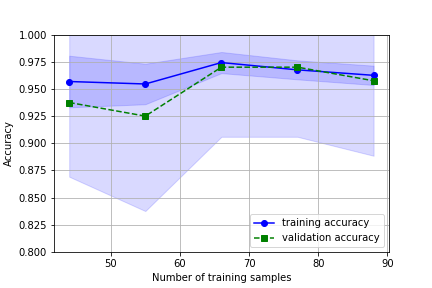
\includegraphics[width=0.5\textwidth]{learning_curve}
  \caption{Learning curve for SVC}
  \label{fig:learning_curve}
\end{figure}

%figure
\begin{figure}[h]
  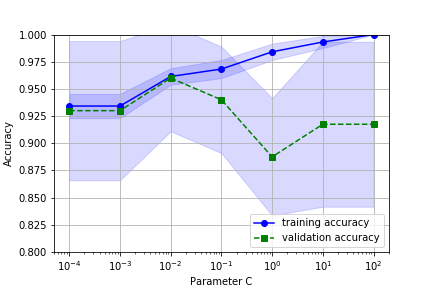
\includegraphics[width=0.5\textwidth]{validation_curve}
  \caption{Validation curve for SVC}
  \label{fig:validation_curve}
\end{figure}

%figure
\begin{figure}[h]
  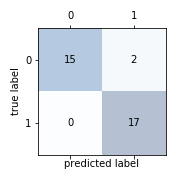
\includegraphics[width=0.33\textwidth]{confusion_matrix}
  \caption{Confusion matrix for SVC}
  \label{fig:confusion_matrix}
\end{figure}

%figure
\begin{figure}[h]
  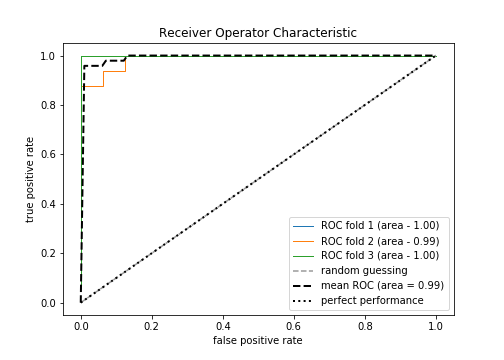
\includegraphics[width=0.5\textwidth]{ROC_curve}
  \caption{ROC curve for SVC}
  \label{fig:ROC_curve}
\end{figure}

\newpage
% Table
\begin{table}%
\caption{SVC performance on single playlist}
\label{tab:one}
\begin{minipage}{\columnwidth}
\begin{center}
\begin{tabular}{ll}
  \toprule
  Test accuracy    & 94.1\%\\
  Recall  & 100\%\\
  Precision    & 88.2\%\\
  F1-score    & 93.7\%\\
  \bottomrule
\end{tabular}
\end{center}
\bigskip\centering
\footnotesize
 \emph{Precision scores for SVC model}
\end{minipage}
\end{table}%
\newpage
We also applied multi-class classification for 9 playlists for which we had more than 50 songs in our dataset. With this modeling technique called one-vs-all classification, one classifier is fitted for each class against all of the other classes. The training set consisted of 718 songs, while the test set included 180 songs. Given the superior performance of the SVC model on one playlist, we optimized it in the multi-class setting using grid search and cross-validation. The grid search for the multi-class SVC yielded a model with training accuracy of 64.5\% and CV accuracy of 54.7\%. Grid search with cross-validation was also performed on a random forest model in order to estimate the number of trees in the forest, the number of features to consider for the best split, the maximum depth of a tree, the minimum number of samples required to split an internal node, the minimum number of samples required for a leaf node, whether bootstrap samples are used and what criterion between Gini impurity and entropy is used for a split. The best random forest model achieved a training accuracy of 68.4\% and cross-validated accuracy of 56.4\%. The test accuracy was 52.2\%. The feature importance from the random forest in order of usefulness can be seen in the plot below. Importance is calculated for each feature from the amount that each split improves the performance criterion, weighted by the number of observations of the node.

%figure
\begin{figure}[h]
  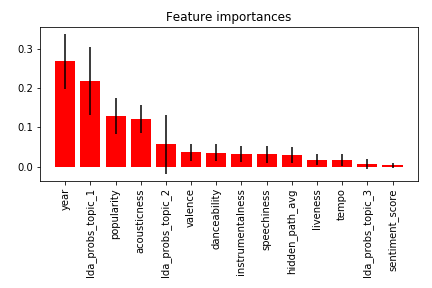
\includegraphics[width=0.5\textwidth]{feature_importance2.png}
  \caption{Figure: Feature importance of random forest for multi-class prediction}
  \label{fig:ROC_curve}
\end{figure}

\newpage

We also applied another technique, employing a random forest classifier and encoding each tree as a feature index in a new high-dimensional feature space. Then we applied a logistic regression model on this sparse, one-hot encoded embedding of the data. The test set accuracy achieved with this method was 51.1\%.
The final technique that was employed was an ensemble method, namely plurality voting, which selects the playlist that received the most votes from the majority of a group of classifiers. The classifiers we implemented for plurality voting were logistic regression, SVC, decision tree, random forest and KNN. The cross-validated accuracy of the plurality voting ensemble was 55\% $\pm$ 2\%. The classifiers' cross-validated accuracy is summarized in table \ref{tab:two}.  
% Table
\begin{table}%
\caption{Cross-validated accuracy of classifiers in plurality voting}
\label{tab:two}
\begin{minipage}{\columnwidth}
\begin{center}
\begin{tabular}{ll}
  \toprule
  Logistic Regression    & $51\% \pm 3\%$\\
  SVC  & $49\% \pm 3\%$\\
  Decision Tree  & $46\% \pm 3\%$\\
  Random Forest  & $55\% \pm 2\%$\\
  KNN  & $48\% \pm 2\%$\\
  Plurality Voting  & $55\% \pm 2\%$\\
  \bottomrule
\end{tabular}
\end{center}
\bigskip\centering
\footnotesize
 \emph{Plurality voting CV performance} 
\end{minipage}
\end{table}%
\newpage

\subsection{Graph}

TODO

Baseline: Avg distance within train set:          0.241749220274
Avg distance of prediction to positive train set: 0.191966891286
Avg distance of prediction to positive test set:  0.196542014849
Avg distance of prediction to negative test set:  0.292054955012

19.0
Avg distance to actual playlist: 0.231436866148

\section{Conclusions}

We are pleased with how both approaches to the task performed, and we attribute the accuracy to the strength of our features, both raw and derived. In particular we saw increased performance when adding popularity and lyrics data. When making a playlists, people choose songs that make them feel a certain way, and lyrics are huge part of that. Also people choose songs that they’ve actually heard of, so popularity is important. Our training data was biased towards popular songs in particular because we chose top results.

% Bibliography
\bibliographystyle{plain}
\bibliography{lit}{}

%\input{samplebody-journals}

\end{document}
